\begin{enumerate}
 \item In the Figure $2$,PQ is a chord of a circle with centre O and PT is a tangent.If $\angle QPT$=$60\degree$,find $\angle PRQ$
  \begin{figure}[h]
      \centering
      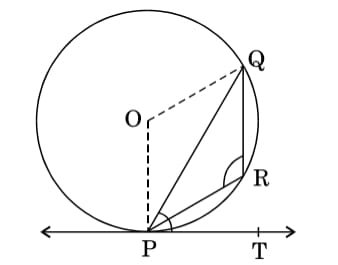
\includegraphics[width=0.6\columnwidth]{figs/cir12.jpg}
  \end{figure}

  \item Prove that the tangent at any point of a circle is perpendicular to the radius through the point of
  contact.

  \item In Figure $3$, two tangents $RQ$ and $RP$ are drawn from an external point $R$ to  the   circle   with   centre   $O$.   If   $\angle PRQ $  =  $120\degree$,  then   prove   that $ OR=PR+RQ $ 
   \begin{figure}[h]
        \centering
           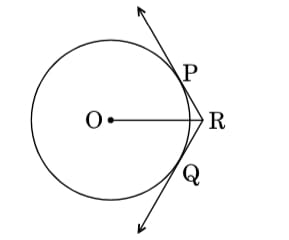
\includegraphics[width=0.6\columnwidth]{figs/cir13.jpg}
       \end{figure}
  \item Prove that the lengths of the tangents drawn from an external point to a circle are equal.
   \item Prove that the tangent drawn at the mid-point of an arc of  a  circle  is parallel to the chord joining the end points of the arc.      
   \item  In  Figure  $4$,  a  triangle  $ ABC $  is  drawn  to  circumscribe  a  circle  of  radius $3$ cm, such that the segments $ BD $ and $ DC $ are respectively of lengths $6$ cm and $9$ cm. If the area of $\triangle ABC$ is $54$ $cm^2$, then find the lengths of sides AB and AC.
    \begin{figure}[h]
       \centering
       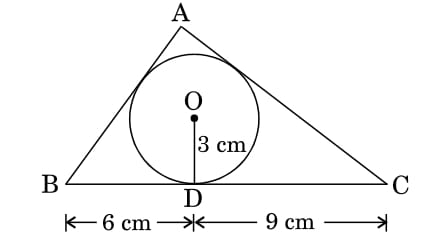
\includegraphics[width=0.6\columnwidth]{figs/cir14.jpg}
    \end{figure}
    \end{enumerate}
